\documentclass[a4paper,12pt]{article}
\usepackage{graphicx,textcomp,amsmath,amssymb,IEEEtrantools,adjustbox,wrapfig,chngcntr,tikz,float,amsthm,listings,caption}
\usepackage[toc,page]{appendix}
\usepackage{hyperref}
\hypersetup{
    colorlinks,
    citecolor=blue,
    filecolor=blue,
    linkcolor=blue,
    urlcolor=blue
}

\usepackage{parskip}
\usepackage{indentfirst}

\usepackage{fancybox} 

\usepackage{fancyhdr}
\pagestyle{fancy}
\fancyhead{}
\renewcommand{\headrulewidth}{0pt}
\usepackage{blindtext}
\usepackage{lastpage}
\rfoot{Page{} \thepage\ of \pageref{LastPage}}
\cfoot{}
\chead{\footnotesize{How do modern cryptographic methods effectively secure online communications, transactions, and the internet?}}

\definecolor{codegreen}{rgb}{0,0.6,0}
\definecolor{codegray}{rgb}{0.5,0.5,0.5}
\definecolor{codepurple}{rgb}{0.58,0,0.82}
\definecolor{backcolour}{rgb}{0.95,0.95,0.92}


\counterwithin{equation}{section}

\usepackage{setspace}
\doublespacing

%BORDER
\usepackage[paperwidth=7.27in,paperheight=10.69in,left=1in, right=1in, top=1in, bottom=1in]{geometry}
\usepackage[a4,frame,center,noinfo]{crop}


\setlength{\parskip}{2em}
\setlength{\parindent}{1cm}

\binoppenalty=10000
\relpenalty=10000

\newtheorem{theorem}{Theorem}
\theoremstyle{definition}
\newtheorem{definition}{Definition}

\begin{document}
\begin{titlepage}
    \begin{center}
    
        \vspace*{1cm}
 
        \Large
        \textbf{Extended Essay}

        
 		\textbf{Subject:} Mathematics
        \vspace{0.2cm}
        
        \textbf{Topic:} Public-Key Cryptography
        \vspace{2.5cm}
		
		
		\textbf{Research Question: }How do modern cryptographic methods effectively secure online communications, transactions, and the internet?
 
        \vfill
 
 
        \vspace{0.8cm}
 
 
        \Large
       \textbf{Word Count: }3952 
 
    \end{center}
\end{titlepage}



\tableofcontents


\newpage
\section{An introduction into modern public-key cryptography}


\indent Throughout history, beginning from the days of the Caesar cipher, individuals have wanted to exchange secret messages. To encrypt and decrypt these messages there has always been a secret \textbf{key} that both ends needed to have. This method is called symmetric cryptography where both the sender and the receiver have to have the same key. This is very dangerous as if a malicious user got a hold of the key, they could decrypt the message very easily.

Modern application use  public key cryptography which is assymetric in nature. That means that the encryption and decryption keys are different. In it, there are two keys. One is public, everyone has it. The other one is private. The encrypted message is secured using a \textit{public key}, and can only be decrypted using a that same user's \textit{private key}. This makes sense that only the intended receiver can decipher a message sent to them with their \textit{private key} if encrypted with that their own \textit{public key}.

Hence, for the purposes of modern cryptography, messages are exchanged without the risk associated with symmetric encryption. This negates the risk associated with a stolen key, making it near impossible for malicious users to decipher messages. So, now it brings us to the question \textbf{``How do modern cryptographic methods effectively secure online communications, transactions, and the internet?"}

\subsection{Public Key Cryptography: A high level overview} \label{publickeyexchange}

Let us define two individuals who want to send each other a secret parcel. Let their names be Alice and Bob wherein Alice is the sender and Bob is the receiver.
\begin{enumerate}
	\item First Bob sends an unlocked padlock to Alice (Bob would send that to anyone even someone he doesn't really trust). This is the \textit{public key}. The only use of an unlocked padlock is to send Bob a parcel since Bob is the only one who has the key that can open the padlock.
	\item Alice locks up the package she wants to send with the padlock Bob sent her. Only Bob can open the package now.
	\item After receiving the package, Bob can open it with his \textit{private key}.
\end{enumerate}

This simple exchange makes the basis of Public Key Cryptography. It involves two \textit{keys}, different one for encryption (padlock) and decryption (key) and is known as the Public Key Exchange\footnote{Ellis, James H. ``The possibility of secure non-secret digital encryption." \textit{UK Communications Electronics Security Group,} 1970.}.
\begin{figure}[h]
	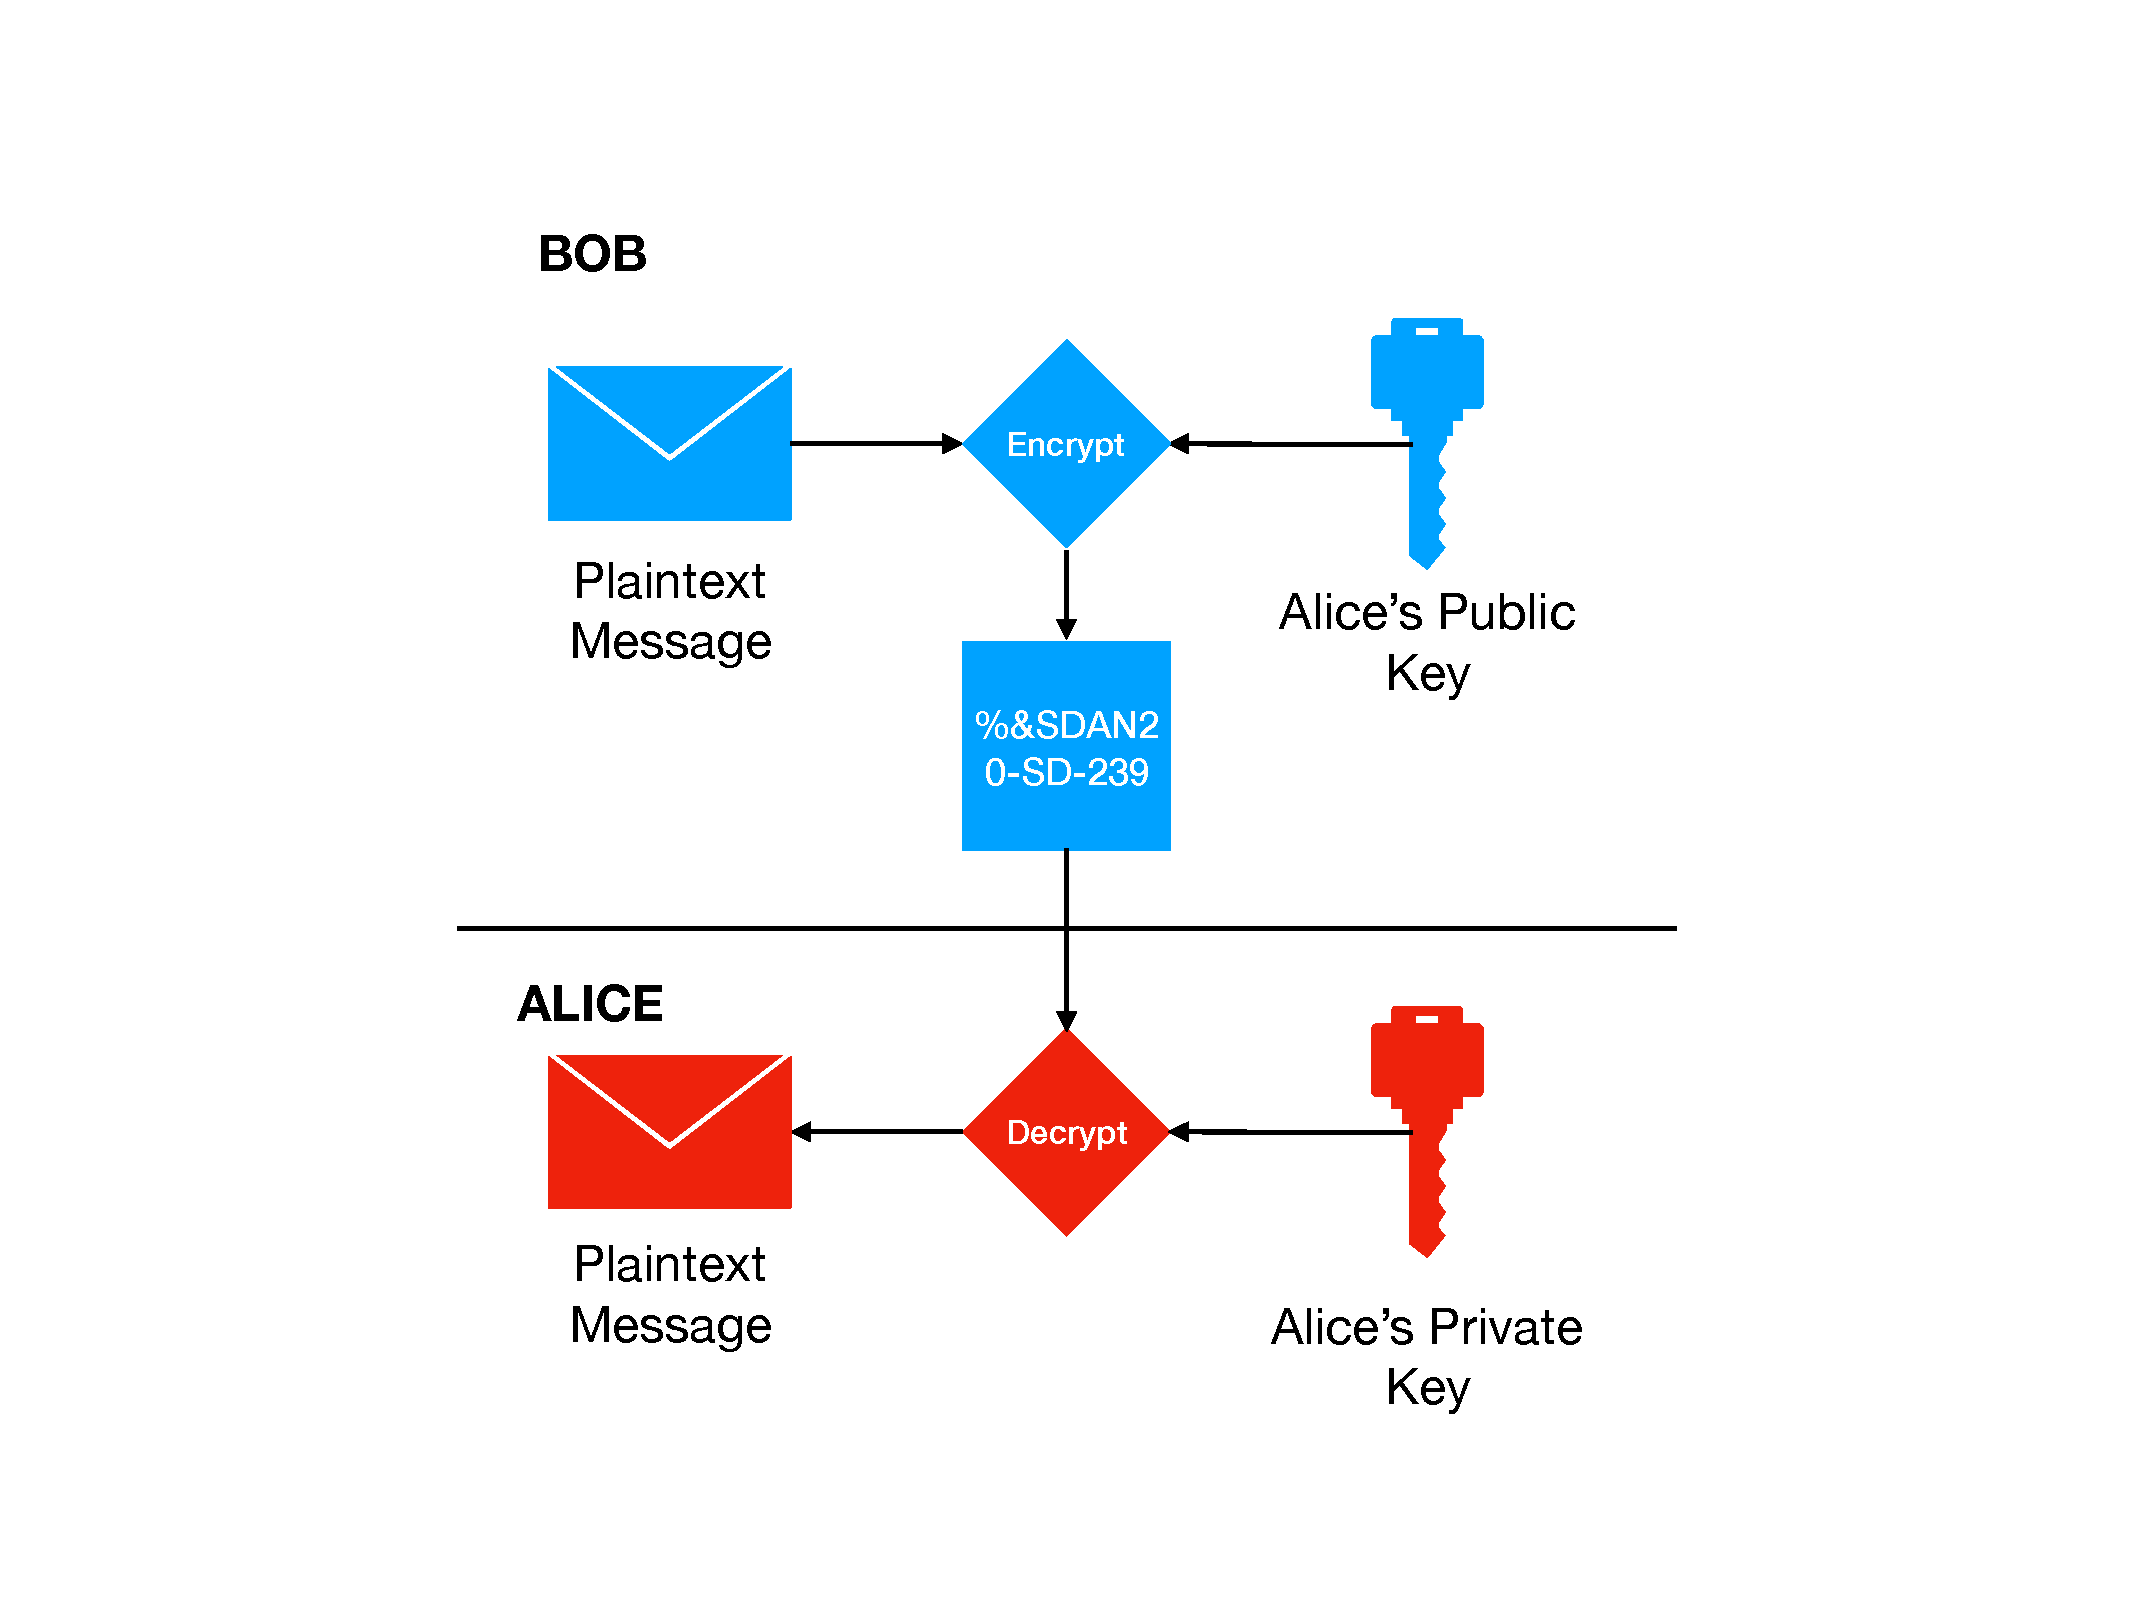
\includegraphics[width=\textwidth]{bobalice}
	\centering
	\caption{Public Key Exchange Visualization}
\end{figure}



\newpage
\subsection{Assumptions in the Public-Key Exchange} \label{assumptions}
If we need to generate these keys we need to assume a few things (they will be explored):
\begin{enumerate}
	\item Generating large prime numbers of a particular bit-size, that is a particular number of digits, is easy.
	\item Multiplying large primes is easy. So if $p,q$ are primes, finding their product $n=p \times q$ is trivial.
	\item With a product of primes $n$, it difficult to recover the prime factors $p$ and $q$.
	\item  It is easy to compute the encrypted text called $Ciphertext$.   Formally this is called modular exponentiation and can be be represented like,
	\begin{equation}
		Encryption(Message) = Ciphertext
	\end{equation}
	\item  The reverse of modular exponentiation -- Modular root extraction -- is easy given the decryption key,
	\begin{equation}
		Decryption(Encryption(Message)) = Message
	\end{equation}
	\item For all other cases modular root extraction is difficult. When a third party gets the encrypted ciphertext and tries to decrypt it, they cannot do it without the decryption key. Therefore, unlike the encryption and decryption key are different and that is why it is termed as Asymmetric Cryptography.
\end{enumerate}

The significance of these operations, to tackle the assumptions, will be explained and explored later in the essay, specifically section \ref{rsamainsection}.

\newpage
\section{Divisibility, modular arithmetic, and number theory}
\subsection{Prime Numbers and factorizing}
Prime numbers, how difficult they are to find, and factor, make the basis of public key cryptography\footnote{Lynn, Ben. ``Number Theory." \textit{Applied Cryptography Group,} Stanford University, crypto.stanford.edu/pbc/notes/numbertheory/crt.html. Accessed on 1 Oct 2018.}. A prime number $p \in \mathbb{Z}^+$ that cannot be formed by multiplying two numbers together with its only factors being 1 and itself.

\begin{theorem}[Euclid's Theorem]
    The set of all prime numbers is infinite\footnote{Euclid, and Thomas Little Heath. \textit{The Thirteen Books of Euclid's Elements.} Vol. 2, Cambridge University Press, 2015.}.
\end{theorem}
Consider a finite list of all the primes,
\begin{equation*}
    p_1=2<p_2=3<p_3=5<...<p_n
\end{equation*}

Where the product of all primes in that list, $P$, is,
\begin{equation*}
    P= p_1 \cdot p_2 \cdot p_3 \cdot ... \cdot p_n
\end{equation*}

Consider $(P+1)$, 
\begin{enumerate}
	\item $(P+1)$ is a prime:  there is at least one more prime.
	\item $(P+1)$ isn't prime: there is some prime $p$ that divides $(P+1)$. Also if $p$ were on the list it would also divide $P$. Hence, it would also have to divide the difference $(P+1) - P = 1$. Since no prime divided 1, $p$ cannot  be on the list since primes on the list divide $P$, so there exists one additional prime $p$.
\end{enumerate}

Both cases show that it is impossible to create a finite list of primes.

Few definitions required for further evaluation:
\theoremstyle{definition}
\begin{definition}{Greatest Common Divisor $(gcd())$:}
	The $gcd(a,b)$ where $a,b \neq 0$ is the greatest possible integer ($\mathbb{Z^+}$) that divides both of the integers $a$ and $b$\footnote{\label{chapter2B}Fannon, Paul et al. ``2B: Greatest Common Divisor and Least Common Multiple." \textit{Mathematics Higher Level for the IB Diploma Option Topic 10 Discrete Mathematics}. Cambridge University Press, 2013, pp. 19-23.}.
\end{definition}
\theoremstyle{definition}
\begin{definition}{Coprime or relatively prime:}
	Let $a$ and $b$ be two integers. They are said to be if $gcd(a,b)=1$, that is, they have no common factors besides $1$\textsuperscript{\ref{chapter2B}}.
\end{definition}


\subsection{Modular Arithmetic}

In modular arithmetic, the modulo function gives the remainder upon division by another number. Two numbers $a$ and $b$ are congruent or equivalent when they give identical remainders upon being divided by a number $n$. Another way to say it would be that they are congruent in modulo $n$ if $(a-b)$ is an $\mathbb{Z^+}$ multiple of $n$, i.e.,
\begin{equation*}
    \frac{(a-b)}{n} = k \in \mathbb{Z^+}
\end{equation*}

For example, when $15$ and $-9$ is divided by $12$, they give the same remainder, therefore,
\begin{equation}
	a \equiv b \pmod{n} \iff n|a-b
\end{equation} 

This could be said to be a linear congruence if $a=qn+r$ and $b=ln+r$, that is,
\begin{equation}
	a \equiv b \pmod{n} \iff \exists\ l,q,r \in \mathbb{Z}: a = qn + r\ and\ b = ln + r
\end{equation}

Similarly, other rules for modular arithmetic\footnote{Fannon, Paul et al. ``5B: Rules of Modular Arithmetic." \textit{Mathematics Higher Level for the IB Diploma Option Topic 10 Discrete Mathematics}. Cambridge University Press, 2013, pp. 53-55.} are as expected,
\begin{equation*}
    \text{if } a \equiv b \pmod n \text{ and } c \equiv d \pmod n \text{ then}:
\end{equation*}

\begin{itemize}
	\item $ac \equiv bc \pmod n$
	\item $a+c \equiv b+d \pmod n$
	\item $a-c \equiv b-d \pmod n$
	\item $a^m = b^m \pmod n$
	\item $ka \equiv kb \pmod n \mbox{ for all } k\in \mathbb{Z}$
\end{itemize}

Division, however, is different\footnote{Fannon, Paul et al. ``5C: Division and Linear Congruences." \textit{Mathematics Higher Level for the IB Diploma Option Topic 10 Discrete Mathematics}. Cambridge University Press, 2013, pp. 56-59.}. Suppose we want to make both sides of a congruence divisible by $d$. We can subtract or add a multiple of $n$ from one side of a congruence. This means the following equation is equivalent,
\begin{equation*}
    a \equiv b \pmod n \equiv  a \equiv b \pm n \pmod n
\end{equation*}
\indent This will allow us to make both sides divisible by $d$. This brings us to the three rules of division. 
\begin{itemize}
	\item Consider when $a \equiv b \pmod n$ and $d$ divides both $a,b$, and $gcd(d,m)=1$, then,
\begin{equation*}
	\frac{a}{d} \equiv \frac{b}{d} \pmod n
\end{equation*}
	For example, if $5x \equiv 15 \pmod{24}$ then $x \equiv 3 \pmod{24}$ as 5 is coprime with 24. 
	\item When $d$ and $m$ have same common factors we need to change the modulo when dividing.  If $a \equiv b \pmod n$ and $d$ divides $a,b,n$ then, 
	\begin{equation*}
		\frac{a}{d} \equiv \frac{b}{d} \pmod{\frac{n}{d}}
	\end{equation*}
	\item If $a \equiv b \pmod n$ and $d$ divides $a,b$ then, 
	\begin{equation*}
		\frac{a}{d} \equiv \frac{b}{d} \pmod{\frac{n}{gcd(d,n)}}
	\end{equation*}
\end{itemize}


\subsection{Fermat's Little Theorem}
\begin{theorem}[Fermat's Little Theorem]
	Let $p$ be a prime number and $a$ any integer. Then $a^p -a$ is always divisible by $p$. It can also be written in modular arithmetic notation as\footnote{``Fermat's Little Theorem." \textit{Brilliant Math \& Science Wiki}, brilliant.org/wiki/fermats-little-theorem/. Accessed on 8 Dec. 2018.}:
\begin{equation} \label{littletheorem}
	a^{p} = p \pmod p \textbf{  or } a^{p-1} = 1 \pmod p 
\end{equation}
\end{theorem}
To prove consider, 
\begin{equation*}
\text{Let, }	a \equiv 0 \pmod p
\end{equation*} 
\begin{equation*}
\text{evidently, } a^p \equiv 0 \pmod p	
\end{equation*}
\begin{equation*}
\text{therefore, }	a^p \equiv a \pmod p
\end{equation*}

So now we only need to prove equation \ref{littletheorem} where $a$ not divisible by $p$. 
Considering the list of the first non-negative numbers $p$ multiplied by $a$,
\begin{equation} \label{fermatslittletheoremlist2}
	0,1,2,3,...,p-3,p-2,p-1
\end{equation}
\begin{equation} \label{fermatslittlethoremlist1}
	\Rightarrow 0,a,2a,3a,...,(p-3)a,(p-2)a,(p-1)a
\end{equation}
Reducing this new list of numbers $\pmod{p}$, will give us the original list, that is, we can use a property of the modulus function.

For the proof\footnote{Burton, David M. \textit{Elementary Number Theory.} 7th ed., McGraw-Hill, Higher Education, 2011.}, let us take $a=4$ and $p=7$. This gives us the original list from \ref{fermatslittletheoremlist2} as 
\begin{equation*}
	\{0,1,2,3,4,5,6\}
\end{equation*}
\indent and the new list from \ref{fermatslittlethoremlist1} as 
\begin{equation*}
	\{0,4,8,12,16,20,24\}
\end{equation*}
\indent If we reduce this list $\pmod{7}$, we get $\{0,4,1,5,2,6,3\}$, with all distinct numbers $\pmod p$. It is also just the original list in a scrambled order.

From \ref{fermatslittlethoremlist1} we get,
\begin{equation*}
    0,a,2a,3a,...,a(p-3),a(p-2),a(p-1)a \text{  \thinspace reduced } \pmod p
\end{equation*}
\indent to a list of $p$ so that every  remainder $(0,1,2,3,...,p-3,p-2,p-1)$, appears a single time, so it is in a scrambled order (the zero entities in this list can be disregarded and removed). Both the lists have equivalent elements $\pmod p$, that means their product is also equivalent  $\pmod{p}$:
\begin{equation}
	a \cdot 2a \cdot ...\cdot a(p-2) \cdot a(p-1) \equiv 1 \cdot 2 \cdot ... \cdot (p-2) \cdot (p-1) \pmod p
\end{equation}
\indent Which can be factorized to,
\begin{equation}
	a^{p-1} \cdot 1 \cdot 2 \cdot ... \cdot (p-2) \cdot (p-1) \equiv 1 \cdot 2 \cdot ... \cdot (p-2) \cdot (p-1) \pmod p 
\end{equation}
\indent By subtracting,
\begin{equation}
	a^{p-1} \cdot 1 \cdot 2 \cdot ... \cdot (p-2) \cdot (p-1)   - 1 \cdot 2 \cdot ... \cdot (p-2) \cdot (p-1) \equiv 0 \pmod p
\end{equation}
\indent or,
\begin{equation}
	(a^{p-1}-1) \cdot 1 \cdot 2 \cdot ... \cdot (p-2) \cdot (p-1)   \equiv 0 \pmod p
\end{equation}

Since all the factors, $1,2,...,p-2,p-1$, are lesser than $p$, they cannot be divided by $p$. Therefore, $a^{p-1} -1$ must be divisible by $p$, which proves another form of equation \ref{littletheorem} :
\begin{equation}
		a^{p-1} -1= 0 \pmod p
\end{equation}

\subsection{Chinese Remainder Theorem} \label{chineseremaindersection}
\begin{theorem}[Chinese Remainder Theorem\footnote{Fannon, Paul et al. ``5D: Chinese Remainder Theorem." \textit{Mathematics Higher Level for the IB Diploma Option Topic 10 Discrete Mathematics}. Cambridge University Press, 2013, pp. 59-62.}]\label{chineseremainder}
	If two numbers $p$ and $q$ are coprime, then the simultaneous linear congruencies,
	\begin{equation*}
		\text{} y \equiv a \pmod p \text{ and } y \equiv b \pmod q
	\end{equation*}
	  have a unique solution,
	  \begin{equation*}
	  	n=\pmod{pq}
	  \end{equation*}
\end{theorem}
For example, let us take the pair of equations,
\begin{equation*}
	    \left.
        \begin{aligned}
            y \equiv 3 \pmod 5\\
            \\
            y \equiv 2 \pmod 3
        \end{aligned}
    \right\}
\end{equation*}
% \begin{figure}[H]
% 	 \centering
%      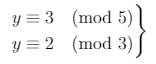
\includegraphics{chineseremainder}
% \end{figure}
\indent That gives us,
\begin{equation*}
	y \equiv 3 \pmod 5 \Rightarrow x=3,8,13,18,23,28,...
\end{equation*}
\begin{equation*}
	y \equiv 2 \pmod 3 \Rightarrow x=2,5,8,11,14,17,20,23,...
\end{equation*}

Doing this is a long process, and we only have 2 solutions, 8 and 23. In the first list, all numbers are +5, in the second list they are +3. So, to get number in both lists we need to +15. Therefore, all solutions are in the form $8+15k$, or $y \equiv 8 \pmod{15}$.




\newpage
\section{The RSA} \label{rsamainsection}
Rivest-Shamir-Adleman abbreviated to RSA\footnote{Rivest, R. L., et al. ``A Method for Obtaining Digital Signatures and Public-Key Cryptosystems." \textit{Communications of the ACM}, vol. 21, no. 2, 1 Jan. 1978.} is a very popular public key cryptosystem used to data transmission on the internet and to secure sensitive transactions. Like introduced in section \ref{publickeyexchange}, it is an asymmetric cipher.

\subsection{Euler's Theorem}

\begin{definition}{Euler's totient function\footnote{Pettofrezzo, Anthony J., and Donald R. Byrkit. \textit{Elements of Number Theory}. Prentice-Hall, 1970, p. 80.}. :}
	$\phi(n)$ denotes the set of numbers $\leq n$ and which are relatively prime to $n$. In other words, $\phi(n)$ is the number of $m \in \mathbb{N}$ such that $1 \leq m < n$ and $gcd(m,n)=1$. It makes the basis of the RSA for the computation of relatively prime numbers required for encryption and decryption.
\end{definition}
Let us take the example of $\phi(12)=4$,

%  \begin{table}[h]
% \centering
% \begin{tabular}{lllll}
% $gcd(1,12)=1$ & & $gcd(5,12)=1$ && $gcd(9,12)=3$ \\
% $gcd(2,12)=2$ & & $gcd(6,12)=6$ && $gcd(10,12)=2$ \\
% $gcd(3,12)=3$ & & $gcd(7,12)=1$ && $gcd(11,12)=1$ \\
% $gcd(4,12)=4$ & & $gcd(8,12)=4$ && $gcd(12,12)=12$ 
% \end{tabular}
% \end{table}
\begin{figure}[H]
	 \centering
     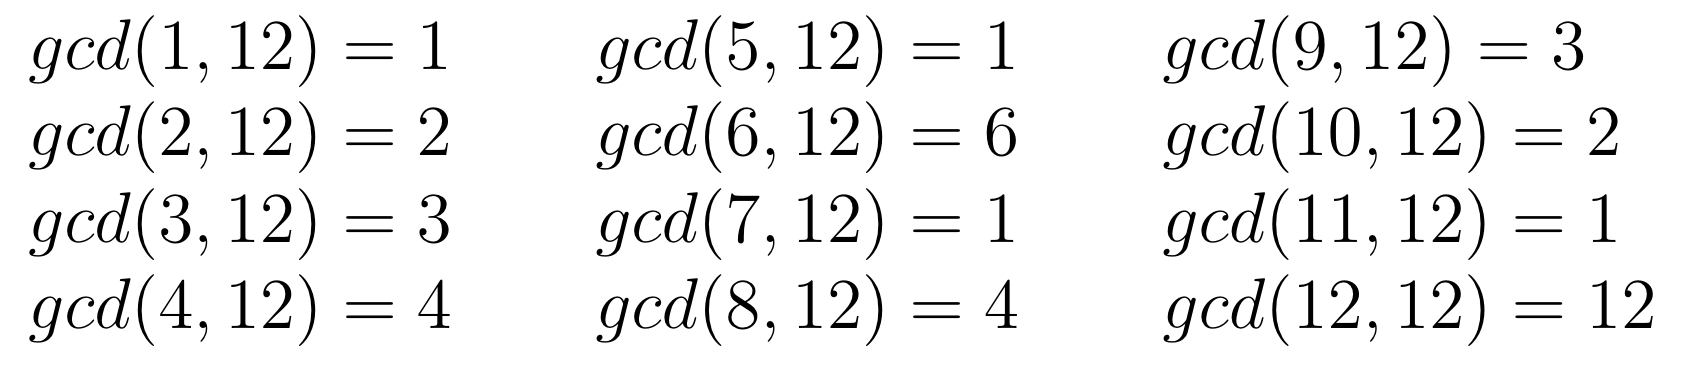
\includegraphics[width=0.8\linewidth]{gcd}
\end{figure}
Therefore for prime $p$,
\begin{equation}
	\phi(p) = p-1
\end{equation}

Since all the integers $\mathbb{Z} < p$ are relatively prime to $p$. The figure \ref{phifigure} for this function till $n=8000$ shows it clearly. There is an evident upper bound of the line $\phi(n) =n-1$
\begin{figure}[H]
	 \centering
     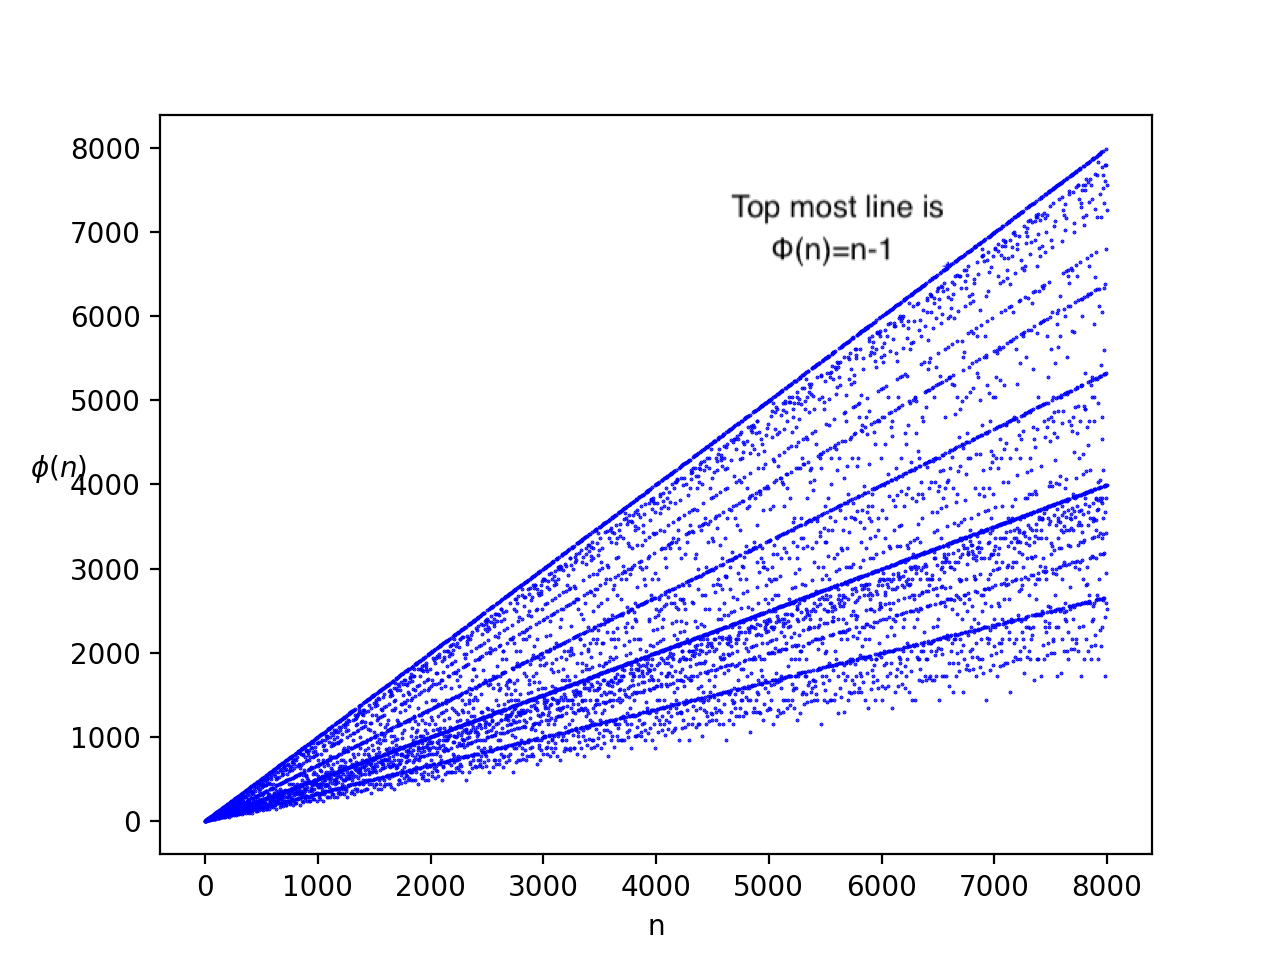
\includegraphics[width=0.7\linewidth]{phi}
     \caption{Graph of $\phi(n)$ for $n \leq 8000$}
     \label{phifigure}	
\end{figure}


\subsection{Encryption Process} \label{rsaencryptionprocess}

The steps taken for encrypting a plaintext message using the RSA are as follows\footnote{Rivest, R. L., et al. ``A Method for Obtaining Digital Signatures and Public-Key Cryptosystems." \textit{Communications of the ACM}, vol. 21, no. 2, 1 Jan. 1978.}:
\begin{enumerate}
	\item Compute two extremely big prime numbers $p$ and $q$ which can be tested for primality (section \ref{primalitytests}).
	\item Compute $n$ where,
		\begin{equation} \label{primeproduct}
			n=p \cdot q
		\end{equation}
	\item Compute $\phi(n)$ where, 
		\begin{equation} \label{phi}
			\phi(n) = (p-1)(q-1)
		\end{equation}
	\item Now, we can disregard $p$ and $q$, such that we erase them from the system in question.
	\item Choose two numbers $e$ (encryption key) and $d$ (decryption key) where $e$ is relatively prime to $\phi(n)$, i.e., $gcd(e,\phi(n))=1$ therefore,
		\begin{equation} \label{ed}
			ed = 1 \pmod{\phi(n)}
		\end{equation}
		Therefore, it complies with Euler's Theorem where $\phi (n)$ is Euler's function which is the amount of numbers smaller than $n$ that are coprime to it. This means that, $(p-1)(q-1)$ is coprime to $n$. The proof for the Little Theorem follows in the next page.
	\item The pair $(e,n)$ makes up the public key, wherein $n$ is called the modulus, and it signifies the number of digits the prime numbers are, and $e$ the exponent.
	\item The private key is $d$ and may sometimes be written as $(d,n).$
	\item Let the plaintext message be $M$ such that $0\leq M \leq (n-1)$. It is possible to convert a message to the decimal system using ASCII values (table in Appendix \ref{app:ascii}). 
	\item To encrypt the plaintext message $M$ to ciphertext $C$, the formula used is,
		\begin{equation} \label{rsaencryption}
			C = M^e\pmod n
		\end{equation}
\end{enumerate}


\subsection{Applying Fermat's little theorem to prove the RSA encryption and decryption} \label{rsaproof}
Fermat's Little Theorem as seen in equation \ref{littletheorem} is\footnote{Kaliski, Burt. ``The Mathematics of the RSA Public-Key Cryptosystem." \textit{Mathematics and Statistics Awareness Month,} Mathaware, www.mathaware.org/mam/06/Kaliski.pdf. Accessed on 15 Oct. 2018.} \footnote{Ouwehand, Martin. ``The (Simple) Mathematics of RSA." \textit{L'Autorité De Certification De L'EPFL,} certauth.epfl.ch/rsa/. Accessed on 15 Oct. 2018.},
\begin{equation}
	a^p \equiv a \pmod p
\end{equation}
Multiplying with $a^{p-1}$,
\begin{equation}
	a^{p-1} \times a^p \equiv a^p \equiv a \pmod p
\end{equation}
Supposing we repeat this multiplication $K$ times,
\begin{equation}
	a^{K(p-1)} \times a^p \equiv a \pmod p
\end{equation}
Regrouping considering $a^p = a^{p-1} \times a$,
\begin{equation}
\begin{split}
	a^{K(p-1)} \times a^{p-1} \times a & \equiv a \pmod p \\
\text{factoring $a^{p-1}$}	\Rightarrow a^{(K+1)(p-1)} \times a &\equiv a \pmod p \\
	\Rightarrow a^{(K+1)(p-1)+1} & \equiv a \pmod p 
\end{split}
\end{equation}
Let $K+1 = N$, since they are both constants,
\begin{equation} 
	a^{N(p-1)+1} \equiv a \pmod p
\end{equation}
Holding true for all $a$ and $N$

From equation \ref{primeproduct}, \ref{phi}, and \ref{ed} we know  $n = p \cdot q$ and $e$ has no common factors with $\phi$. Then we calculate the multiplicative inverse of $e \pmod{\phi}$, i.e. the number $d$, which is the decryption key. Giving, $ed = 1 +$ a multiple of $\phi$ represented as $L(\phi)$, 
\begin{equation} \label{fermatslittle2}
	ed = L(\phi) +1
\end{equation}

From equation \ref{rsaencryption} we know that,
\begin{equation} 
	C = M^e\pmod n
\end{equation}
\indent Here $C$ is the ciphertext made from plaintext $M$. Decryption will require calculation of $z  \equiv C^e \pmod n \equiv M^{ed} \pmod n$. This means the plaintext $z$ is the original message $M$ again. To prove this, we can use equation \ref{fermatslittle2} and \ref{rsaencryption}, and taking $n=pq$,
\begin{equation}
	M^{ed} = M^{L(\phi) +1} \equiv M \pmod p
\end{equation}
\begin{equation}
	\Rightarrow M^{ed} - M = \mbox{multiple of }p
\end{equation}
and the same of $q$ instead of $p$ such that, 
\begin{equation}
		M^{ed} = M^{L(\phi) +1} \equiv M \pmod q
\end{equation}
\begin{equation}
	\Rightarrow M^{ed} - M = \mbox{multiple of }q
\end{equation}
\indent Therefore, $M^{ed} -M$ can only be a multiple of the primes $p,q$ if it is a multiple of $n$, its product. Implying the equation mentioned above using the theorem \ref{chineseremainder} which is the Chinese Remainder Theorem mentioned in section \ref{chineseremaindersection},
\begin{equation}
	M^{ed} \equiv M \pmod n
\end{equation}
\indent This equivalence only establishes the fact that $M^{ed}$ and $M$ have the same remainders $\pmod n$. Since $0<M<n$, the remainder of dividing $M^{ed} \mid n$ is always $M$. Therefore, to recover $M$, $C^e \pmod n$ must be computed.

The public key is the pair $(e,n)$. But, for decryption you need $d$ (private key) and to compute,

\begin{equation} \label{rsadecryption}
	C^d \pmod n \equiv M
\end{equation}

Even though $(e,n)$ is public knowledge, $\phi$ is not, so $d$ cannot be calculated since it is the multiplicative inverse of $e \pmod{\phi(n)}$. $n$ is public knowledge though, but it is not factored into $p,q$. As stated, RSA is safe because of the near impossible problem that is prime factorization of large prime numbers. Therefore since factoring $n$ into $p,q$ is almost impossible, it is nearly impossible to get $\phi = (p-1)(q-1)$ and consequently $d$, making RSA safe.

\subsection{Example RSA encryption}
Following the steps in section \ref{rsaencryptionprocess} we can take a simple example with small prime numbers to show how RSA is securely encrypted.
\begin{enumerate}
	\item Let, $p=7$ and $q=11$
	\item Therefore, $n=7 \times 11 = 77$
	\item So, $\phi(77)=(7-1) \times (11-1) = 60$
	\item Disregarding $p$ and $q$...
	\item We need to find a which satisfies the condition for in equation \ref{phi}, that is, to a number with two prime factors $ed$, and is equivalent to $1 \pmod{\phi(n)}$. The following are numbers which equal $1 \pmod{\phi(77)}$ or $1 \pmod{60}$, but they must be tested for factors:
\begin{table}[h]
\centering
\begin{tabular}{lllll}
61  & 121 & 181 & 241 & 301 \\
361 &  421   & 481    & 541    & 601    \\
 661   &  721   &  781   & 841    & 961     \\
1021    & 1081    &1141     & 1201    & 1261 \\
1321 & 1381 & 1441 & 1501 & 1561 \\
1621 & 1681 & 1741 & 1801  
\end{tabular}
\end{table}
	 \\\\ For the purpose of this example let us take 481 (although it does not matter), therefore,  $e=37$ and $d=13$ since $13 \times 37 = 481$ and $481 \pmod{60}=1$
	\item $(37,77)$ is sent out as the public key
	\item $(13,77)$ is kept as the private key
\end{enumerate}
Now, we must convert our message into a number from 1 to $(n-1)$. Let us take the message ``IB" in ASCII is 73 66. That is,
\begin{equation*}
	I=73
\end{equation*}
\begin{equation*}
	B=66
\end{equation*}
To encrypt we use equation \ref{rsaencryption}, written in code in the Appendix A, 
\begin{equation*}
	73^{37} \pmod{77} 
\end{equation*}
\begin{equation*}
	\Rightarrow 17 \equiv 73^{37} \pmod{77} 
\end{equation*}
and,
\begin{equation*}
	66^{37} \pmod{77} 
\end{equation*}
\begin{equation*}
	\Rightarrow 66 \equiv 66^{37} \pmod{77} 
\end{equation*}
Therefore $C = $ $17$ $66$.

Decrypting using equation \ref{rsadecryption},
\begin{equation*}
	17^{13} \equiv 73 \pmod{77}
\end{equation*}
and,
\begin{equation*}
	66^{13} \equiv 66 \pmod{77}
\end{equation*}
Giving our original message in ASCII  as 73 66.This encryption and decryption method has been mathematically proven in section \ref{rsaproof}

\subsection{Primality Tests} \label{primalitytests}
RSA relies on very large prime numbers for its keys. Due to the inherent nature of prime numbers, there is no such formula that has been devised that can give us a list of primes below $n$. This is what makes the RSA secure as it is very difficult to factor $n$ into $p,q$. Therefore, the best way of finding primes is testing each number for whether it is prime or not. For smaller numbers this is easy, but for larger numbers it is quite difficult, therefore primality tests are used. There are various primality tests such as Miller-Rabin Test and Fermat's test\footnote{Bressoud, David M. ``The RSA Public Key Crypto-System." \textit{Factorization and Primality Testing Undergraduate Texts in Mathematics,} 1989,.} used to do this but for the purpose of this essay they will not be explored. Regardless of primality tests, RSA is still very secure.


\newpage
\section{Elliptical Curve Cryptography}
For applications\footnote{Amara, Moncef, and Amar Siad. ``Elliptic Curve Cryptography and Its Applications." \textit{International Workshop on Systems, Signal Processing and Their Applications, WOSSPA,} May 2011.} on the Internet and Blockchain such as securing digital currency and transactions like Bitcoin, ECC or Elliptical Curve Cryptography might seem like better than RSA  due to two smaller bit sizes, that is a smaller $n$, while simultaneously being harder to crack\footnote{Bauer, Johannes. ``Elliptic Curve Cryptography Tutorial." \textit{Johannes Bauer}, www.johannes-bauer.com/compsci/ecc/. Accessed on 19 Sept. 2018.}. Appendix C shows a comparison in the bit-sizes required for an equivalent security level in both RSA and ECC.
\subsection{Introduction} \label{eccintro} 
Elliptical curves are curves with the formula\footnote{Corbellini, Andrea. ``Elliptic Curve Cryptography: a Gentle Introduction." \textit{Andrea Corbellini Atom,} andrea.corbellini.name/2015/05/17/elliptic-curve-cryptography-a-gentle-introduction/. Accessed on 24 Sept. 2018.}:
\begin{equation} \label{ellipticalcurve}
	y^2 =x^3 + ax + b  \pmod p \text{ for all } a,b \in F_p 
\end{equation}
Here $y,x,a,b$ are all within $F_p$ wherein can be any finite field $F_p:$ in any modulo $p$ domain $\mathbb{Z}/p\mathbb{Z}$. In this modulo field, we may define subgroup by restricting the domain of the elliptical curve. 
\begin{definition}{Subgroup: }
  A subset $H$ of a group $G$ is a subgroup of $G$ if $H$ is itself a group under the operation in $G$ \footnote{Rodin, Altha. “Subgroups.” \textit{M328K,} University of Texas, Aug. 2000, web.ma.utexas.edu/users/rodin/343K/Subgroups.pdf.}.     
\end{definition}



\subsection{Singularity case}
Another condition is that the coefficients must be such that they avoid a singularity. A singular curve cannot be used for the purposes of Elliptical Curve Cryptography. In the diagrams\footnote{Davis, Tom R. ``Elliptic Curve Cryptography." \textit{Mathematical Circles} Topics, 3 Nov. 2013, www.geometer.org/mathcircles/ecc.pdf. Accessed on 9 Jan. 2018.} given beneath the  the blue curve is that of $y^2 =x^3 +ax +b$ purple curve is that of $y=x^3 + Ax +B$. For us to take a square root, $x^3+ax+b \geq 0$. Therefore there is no blue curve when the purple line is negative. So, all blue curves include both the positive and negative values of the square root. A singularity occurs when the purple curve is tangent to the $x$-axis.
\begin{figure}[H]
	 \centering
     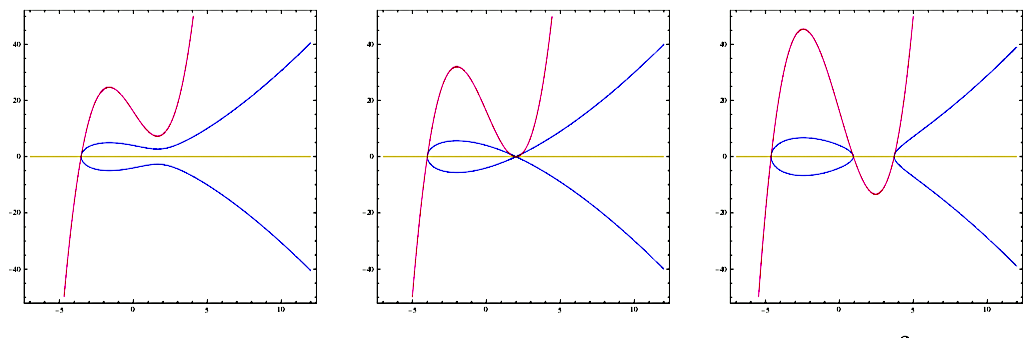
\includegraphics[width=\textwidth]{singularity}
     \caption{Singularity on elliptical curve}
     \label{}	
\end{figure}
The point of tangency will exist where the minimum of the curve $y=x^3 + Ax +B$, the purple line, is on the $x$-axis. 

That is when:
\begin{equation*}
	 \frac{dy}{dx} = 0
\end{equation*}
Taking the derivative of $y=x^3 + Ax +B$,
\begin{equation*}
	\frac{dy}{dx} = 3x^2 + A =0
\end{equation*}
\begin{equation*}
	\text{For} \; x= \sqrt{\frac{-A}{3}} \; \text{to be touching the $x$-axis, we need:}
\end{equation*}
\begin{equation*}
	\left(\sqrt{\frac{-A}{3}}\right)^3 +\left(\sqrt{\frac{-A}{3}}\right)A + B=0
\end{equation*}
\begin{equation*}
	\sqrt{\frac{-A}{3}}\left(\frac{-A}{3}+A\right)=-B
\end{equation*}
\begin{equation*}
		\sqrt{\frac{-A}{3}}\left(\frac{2A}{3}\right)=-B
\end{equation*}
\begin{equation*}
	\frac{-4A^3}{27}=B^2
\end{equation*}
\begin{equation} \label{singularitycase}
	0=4A^3+27B^2
\end{equation}

From equation \ref{singularitycase} we can see that if $4A^3+27B^2=0$ then there is a singularity,  so the properties discussed in section \ref{properties} will not be valid. Therefore, we cannot use a curve with a singularity for ECC.

Hence from now on we will assume the one condition the coefficients of elliptical curves must follow is that:
\begin{equation}
		 4A^3+27B^2 \neq 0
\end{equation}

\subsection{Group Operations} \label{properties}
Elliptical curves have many properties that are useful to making it so secure which are based on the ideas\footnote{Singh, Soram Ranbir, et al. ``A Critical Review on Elliptic Curve Cryptography." \textit{International Conference on Automatic Control and Dynamic Optimization Techniques (ICACDOT),} Sept. 2016.}:
\begin{itemize}
	\item A line that is tangent to the curve but also not a vertical line will always intersect precisely one more point, a third point.
	\item Elliptical curves exist in projective planes. They have a property wherein there exist imaginary points at infinity represented by $\mathcal{O}$. For the purpose of cryptography, $\mathcal{O}$ is an artificial point or zero point that exists ``at infinity" at the coordinates $(0,1,0)$ and will form a vertical line (the reason to why this point exists is out of the scope of this essay).
\end{itemize}

Using these properties we can define two group operations\footnote{Davis, Tom R. ``Elliptic Curve Cryptography." \textit{Mathematical Circles} Topics, 3 Nov. 2013, www.geometer.org/mathcircles/ecc.pdf. Accessed on 9 Jan. 2018.}:

\textbf{Point Addition:}  As shown in the image below, $P + Q = R$ is represented as the reflection on the $x$-axis of the third intersecting point $R'$ of line $PQ$ with the elliptical curve.
\begin{figure}[H] \label{pointadditionimage}
	 \centering
     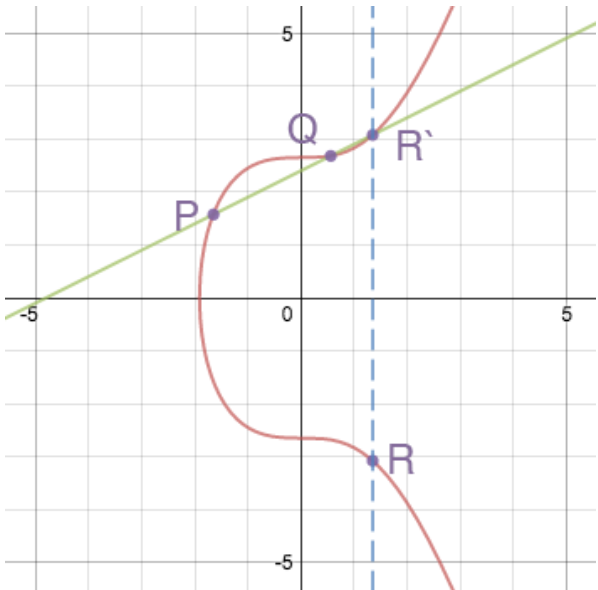
\includegraphics[width=.5\linewidth]{pointaddition}
     \caption{Point Addition}
     \label{}	
\end{figure}

For all $P, Q$, and $R$ in $F_p$, we have the following addition properties, taking from the properties of $F_p$ defined in subsection \ref{eccintro}:
\begin{equation*}
\begin{split}
	P+Q &= Q+P \\
	P+ \mathcal{O} &=P \\
	\mathcal{O} + \mathcal{O} &= \mathcal{O} \\
	P+ (Q+R) &= (P+Q)+R \\
\end{split}	
\end{equation*}

It also shows us that point doubling, explained below, is a special case of point addition wherein $P$ is getting added to itself.

To algebraically derive the coordinates of $R$ let  $PQ$ be linear equation in the form $y=mx+c$. Like all other linear equations, $m$ is the gradient and $c$ is the y-intercept. Let the point $P$ have coordinates $(x_P,y_P)$ and the point $Q$ have the coordinates $(x_Q,y_Q)$. For the case where $P \neq Q$,
\begin{equation}
	m = \frac{y_P - y_Q}{x_P - x_Q}
\end{equation}
\indent Finding the intersection of the line $PQ$ and the elliptical curve,
\begin{equation}
	(mx+y_P)^2=x^3+Ax+B
\end{equation}
\indent Since $(x_P,y_P)$, $(x_Q,y_Q)$, and $(x_R,y_R)$ are all solutions,
\begin{equation}
	\begin{split}
		(x-x_P)(x-x_Q)(x-x_R) &= 0 \\
		x^3 - x^2(x_P + x_Q + x_R) + x(x_Px_Q+x_Qx_R+x_Px_R)-x_Px_Qx_R &= 0
	\end{split}
\end{equation}
\indent Matching coefficients gives us the following coordinates for $R$ as $(x_R,y_R)$,
\begin{equation}
	\begin{split}
		x_R&=m^2-(x_P+x_Q)\\
		y_R&=m(x_P-x_R)-y_P
	\end{split}
\end{equation}


\textbf{Point Doubling:} is Finding the line tangent to the point to be doubled, $P$, and then reflecting the intersecting point $R'$ through the $x$-axis on the curve to get $R$. Represented as $P + P = R = 2P$.
\begin{figure}[!htb]
     \centering
     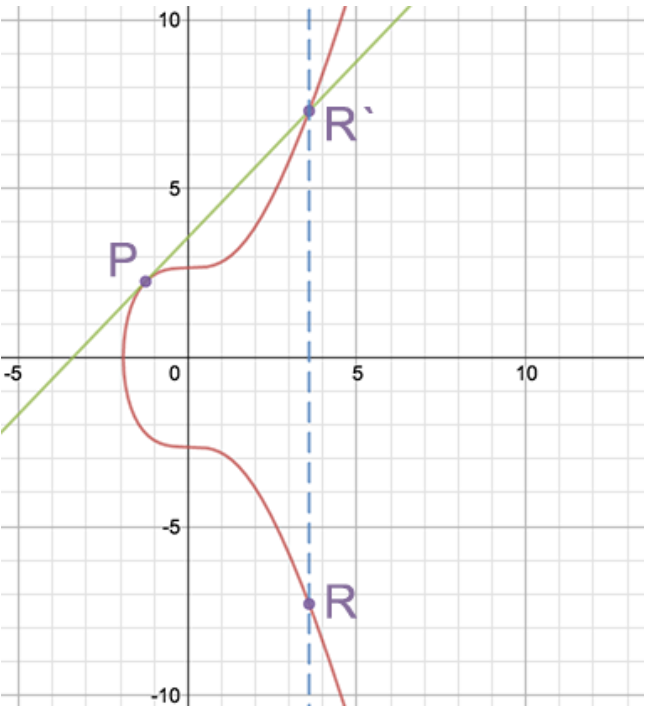
\includegraphics[width=.5\linewidth]{pointdoubling}
     \caption{Point Doubling}
     \label{}
\end{figure} 

For when $P=Q$, like in the case of Point Doubling, we can just take the derivative of the elliptical curve function (equation \ref{ellipticalcurve}) at $(x,y)$,
\begin{equation}
	\begin{split}
		\frac{d}{dx}(y^2) &= \frac{d}{dx}(x^3 +ax+b) \\
		\frac{dy}{dx}(2y) &= 3x^2+a \\
		\frac{dy}{dx} &= \frac{3x^2+a }{2y}
	\end{split}
\end{equation}
\indent That means, if $P=Q$ at $(x_P,y_P)$, then the gradient $m$ at that point is,
\begin{equation} \label{pointdoublingformula}
	m = \frac{3x_P^2+a }{2y_P} 
\end{equation}
\indent Which makes the coordinates of point $R$, $(x_R,y_R)$,
\begin{equation} \label{pointdoublingcoordinates}
	\begin{split}
		x_R &= m^2 -2x_P \\
		y_R &= m(x_P - x_R)-y_P
	\end{split}
\end{equation}

There is sometimes a special case of Point Addition or Point Doubling, when two points create a vertical point. 

\begin{figure}[!htb]
	 \centering
     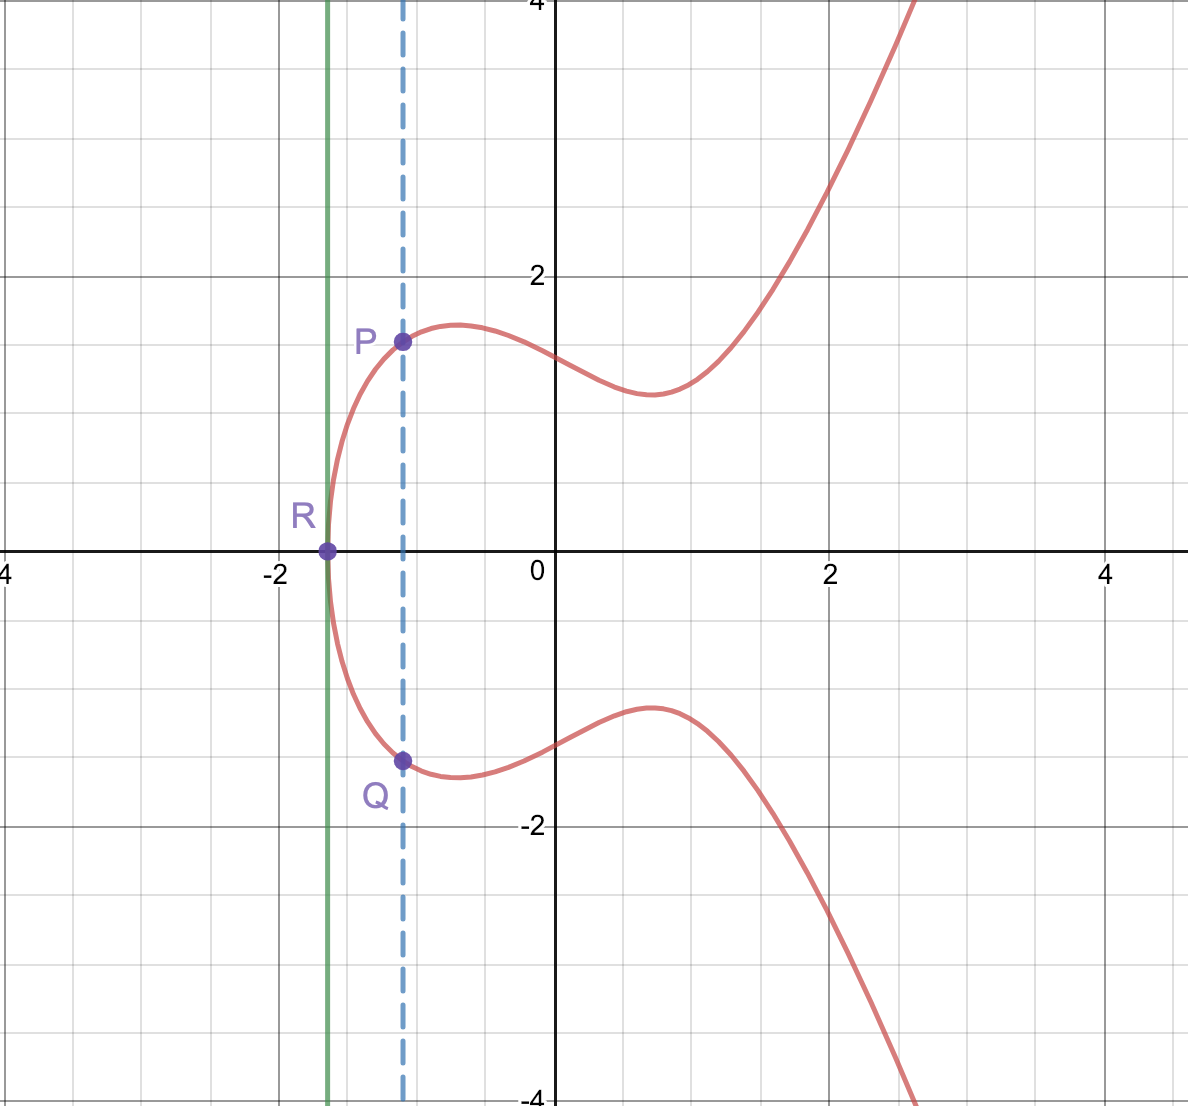
\includegraphics[width=.6\linewidth]{verticalpoint2}
     \caption{Vertical Point}
     \label{verticalpointfigure}	
\end{figure}

The phenomenon shown in figure \ref{verticalpointfigure} happens in two cases:
\begin{enumerate}
	\item When $P \neq Q$ and $x_P =x_Q$, $\Rightarrow P+Q= \mathcal{O}$
	\item If $P=Q$ (represented by point $R$ in figure \ref{verticalpointfigure}) and $y_P=y_Q=0$ then $P+Q= \mathcal{O}$
\end{enumerate}

Together these properties can be used for Scalar Multiplication $R = k\cdot P$ which is defined by $R = P + P + P$ (when $k = 3$), a number of times. This brings us to the definition of $G$ known as the The Base Point or Generator Point such that for any point $G$ on the curve, the set of all the points on that curve is $\{\mathcal{O},G,G+G,G+G+G,...\}$ and is called a cyclic subgroup of the points on the elliptical curve.
\begin{definition}{The Base Point or Generator Point:}
	$G \in E(\mathbb{Z}/p\mathbb{Z})$ where $E$ is an elliptical curve modulo $p$ that generates a cyclic subgroup. That is, any point in the subgroup (a subset of all the points on the curve) can be computed through repeat addition of $G$\footnote{Yin, Xinchun, and Jinliang Zou. ``A Parallel Base Point Choosing Algorithm of ECC on Binary Field." \textit{International Conference on Systems and Informatics (ICSAI2012)}, May 2012.}
\end{definition}
\textbf{Properties of the Generator Point:}
\begin{itemize}
	\item Order of the generator point: $ord(G)$ = $n$, is the number of points that the generator point can make through repeated addition. It is also the smallest possible integer $k$ such that $kG=\mathcal{O}$
	\item Cofactor: $h=\frac{|E(\mathbb{Z}/p\mathbb{Z})|}{n}$, that is the total number of elements in all groups (all points on the curve) divided by $ord(G)$. A cofactor of $n=1$ is ideal since larger cofactors are more susceptible to attacks and are undesirable.
\end{itemize}
The methods used to find the generator point are beyond the scope of this essay as they involve the Lagrange Theorem and Group Theory.

\subsection{Elliptical Curve Discrete Logarithm Problem} \label{ECDLP}
How do we go from this idea of an elliptical curve to a crytosystem that can secure everything on the internet? Looking at the assumptions in section \ref{assumptions} gives us a hint. Using a one-way encryption function, also known as a trapdoor function, makes ECC secure since it allows one operation to be computed easily but the reverse is difficult. That is why it is easy to encrypt a message but very difficult to decrypt it. We have already encountered this in the idea of scalar multiplication.

\begin{definition}{Elliptical Curve Discrete Logarithm Problem (ECDLP):} 
	For an elliptical curve $E$ over a finite field $K_p$. Given a point  $Q \in E(K)$ and generator point $G$, it is currently computationally infeasible to compute $k$ such that $Q=kG$ where $k$ is the discrete logarithm of $Q$ to the base $G$\footnote{Smart, N. P. ``The Discrete Logarithm Problem on Elliptic Curves of Trace One." \textit{Journal of Cryptology}, vol. 12, no. 3, June 1999, pp. 193-196.}
\end{definition}
What makes ECDLP so difficult to crack is the one-way nature of scalar multiplication regarding elliptical curve $\mathbb{E}$ in the finite field $F_p$. This one-way function or trapdoor function that secured the RSA was the factoring of primes, and for ECC it is the ECDLP. These two trapdoor or one-way functions are the basis for the security of the internet. Although primality testing has allowed for some progress to be maid when factoring prime numbers. On the other hand, there has been no such revolutionary progress for the ECDLP.

\subsection{Elliptical Curve Diffie-Hellman protocol key exchange with an example}
Domain parameters are represented as $\{p,a,b,G,n,h\}$ and are the parameters available to both parties exchanging messages and to any third parties since it is on the public domain. An elliptical curve $E$ is used for this process.
\begin{itemize}
	\item $p$: field modulus of the curve $E$ as defined over $\mathbb{Z}/p\mathbb{Z}$.
	\item $a,b$: curve parameters of $E$
	\item $G$: Generator Point
	\item $n$: $ord(G)$
	\item $h$: cofactor
\end{itemize}

Let us compute an example curve and all the parameters before beginning with the process\footnote{Pierce, Robert. ``Elliptic Curve Diffie Hellman," \textit{YouTube,} 10 Dec. 2014, www.youtube.com/watch?v=F3zzNa42-tQ. Accessed on 3 Jan. 2019.}.

	For the purpose of the example let,
	\begin{equation} \label{sampleellipticalcurve}
		E: y^2 \equiv x^3 +2x+2 \pmod{17}
	\end{equation} and therefore $G=(5,1)$. Such small numbers are never used since they are not secure, but to illustrate the example it  is sufficient.
	
	Now we need to generate the cyclic group using $G$. The first step is to compute $2G$ which is $G+G$. To do this we can use the point doubling formula derived in equation \ref{pointdoublingformula}:
	\begin{equation}
		m = \frac{3x_G^2+a }{2y_G} 
	\end{equation}
	Since $G=(5,1)$, $x_G=5$ and $y_G=1$ and $a=2$ from \ref{sampleellipticalcurve}:
	\begin{equation}	
			m \equiv \frac{3(5^2)+2 }{2(1)} \equiv \frac{77}{2}  \equiv77 \cdot 2^{-1} \equiv 9 \cdot 9 \equiv 13 \pmod
		{17}
	\end{equation}
	\textit{Note: $2^{-1} \pmod{17} \equiv 9$ was computed using the Extended Euclidean Algorithm which is outside the mathematical scope of this essay.}
	
	Next, we compute the $x_{2G}$ and $y_{2G}$ coordinates for $2G$ using the formula in \ref{pointdoublingcoordinates}
	\begin{equation}
		x_{2G}=m^2 - 2x_G
	\end{equation}
	\begin{equation}
		x_{2G} \equiv 13^2 -2(5) \equiv 169 - 10 \equiv 16 - 10 \equiv 6 \pmod{17}
	\end{equation}
	and,
	\begin{equation}
		y_{2G} = m(x_G -x_{2G}) - y_G
	\end{equation}
	\begin{equation}
		y_{2G} \equiv 13(5-6) - 1 \equiv -13-1 \equiv-14 \equiv 3 \pmod{17}
	\end{equation}
	The coordinates of $2G$ are $(6,3)$. Just like this we need to compute the whole cyclic group till the last point $\mathcal{O}$. The cyclic group for our $E$ and $G$ is:
	
\begin{table}[h]
\centering
\begin{tabular}{lllll}
$G=(5,1)$   & $5G=(9,16)$  & $9G=(7,6)$    & $13G=(16,4)$  & $17G=(6,14)$      \\
$2G=(6,3)$  & $6G=(16,13)$ & $10G=(7,11)$  & $14G=(9,1)$   & $18G=(5,16)$      \\
$3G=(10,6)$ & $7G=(0,6)$   & $11G=(13,10)$ & $15G=(3,16)$  & $19G=\mathcal{O}$ \\
$4G=(3,1)$  & $8G=(13,7)$  & $12G=(0,11)$  & $16G=(10,11)$ &                  
\end{tabular}
\end{table}

We find that $n=19$ and $h=1$ by counting the number of points in this subgroup.

We are using the Elliptical Curve Diffie-Hellmann exchange since it is the most popular but other protocols are also in use today. The process for ECDH follows the typical public-key exchange structure we saw in section \ref{publickeyexchange} with Bob and Alice:
\begin{enumerate}
	\item Bob picks a private key such $\beta$ such that $1 \leq \beta  \leq n-1$ and computes the point $B=\beta G$ through scalar multiplication and which lies on the curve $E$. Let $\beta = 9$ then $B=9G =(7,6)$.
	\item Alice picks a private key such $\alpha$ such that $1 \leq \alpha  \leq n-1$ and computes the point $B=\alpha G$ through scalar multiplication and which lies on the curve $E$. Let $\alpha =3$ then $A=3G=(10,6)$.
	\item Bob and Alice swap the information about $A = (x_A,y_B)$ and $B = (x_B,y_B)$. This information is made public and acts as the public keys. However, this does not give the public information about $\alpha$ and $\beta$ due to the ECDLP explained in section \ref{ECDLP}.
	\item Alice multiplies Bob's point with her private key $P=\alpha \times B= \alpha \beta G$. This gives Alice $\alpha B = 3B = 3(9G) = 27G = 8G = (13,7)$. Here $27G$ reduces to $8G$ since the order of the cyclic group was $n=19$.
	\item Bob multiplies Alice's point with his private key $P=\beta \times A= \beta \alpha G$. Similar to Alice, Bob computes $(13,7)$
	\item Bob and Alice now have the same point on the curve $P$ that no one else has. They are free to use this information as they wish. For example, they can use the $x$-coordinate to encrypt messages. This is very secure since no third party has access to $\alpha$ or $\beta$ and therefore cannot compute the point $P$ due to the ECDLP.
\end{enumerate}

\newpage
\section{Conclusion}


Digital packets or messages make up all major internet processes. When we visit a website, buy something using a credit card, or send cryptocurrency over the internet, all our information is \textit{encrypted} into these digital messages before being sent. As we have seen, RSA and ECC are two methods to secure these digital messages. \textbf{Do RSA and ECDH effectively secure digital packets?}

Going back to the assumptions in section \ref{assumptions}, we can see that what we needed to assume as true allows these protocols to be secure. If someone wanted to decipher a message encrypted using the RSA, they would need the decryption key $d$. From the encryption process of the RSA (section \ref{rsaencryptionprocess}) we know that $e$ and $n$ are shared as the public key to allow anyone to send the receiver a message.. To compute $d$ from $e$ and $n$ is only possible if someone knew $\phi(n)$. Without the knowledge of the two very large primes $p,q$, it is very difficult to get $\phi(n)$. Intuitively, one would try to factor $n$ into $p$ and $q$. This is very difficult as one has to check for every number from 0 to $\sqrt{n}$ until they find $p$ or $q$. For RSA key sizes which are usually 1024 to 2048 digits long (see Appendix B), this would take years and years, even for the fastest supercomputers. Another way to do it would be count the integers less than $n-1$ which satisfy $gcd(integer,n)=1$. With modern RSA standards using $n$ at least as large as $2^{1024}$, this would take many years even with the fastest supercomputers.

On the other hand, ECDH, a protocol of ECC, is secure not only because of the difficulty of factoring large primes but also due to the ECDLP (section \ref{ECDLP}). There have been various attempts to partially solve this problem like baby-step-giant-step, Pollard rho and kangaroo, index calculus, and summation polynomials are all techniques used\footnote{Galbraith, Steven D. and Pierrick Gaudry. ``Recent progress on the Elliptic Curve Discrete Logarithm Problem. \textit{Designs, Code, and Cryptography,} vol. 78, no. 1, 23 Nov. 2015, pp. 51-72.} but nothing that makes ECC unusable for even the most secure application. Furthermore, as seen in Appendix C, ECC can make use of smaller bit-sizes and provide and equivalent security to RSA. Therefore, the persistence of RSA is only due to the ubiquity of public key infrastructure that supports it, such as in modern browsers. Newer applications like cryptocurrency (and other 
applications of blockchain protocols) often do choose to use ECC rather 
than RSA for authentication, but for existing applications the switching 
costs are high.




\cleardoublepage
\textbf{\Large Works Cited}
\begin{flushleft}
\hangindent0.5in
\sloppy
\textbf{\large Print}

Amara, Moncef, and Amar Siad. ``Elliptic Curve Cryptography and Its Applications." \textit{International Workshop on Systems, Signal Processing and Their Applications, WOSSPA,} May 2011.

Bressoud, David M. ``The RSA Public Key Crypto-System." \textit{Factorization and Primality Testing Undergraduate Texts in Mathematics,} 1989.

Burton, David M. \textit{Elementary Number Theory.} 7th ed., McGraw-Hill, Higher Education, 2011.

Euclid, and Thomas Little Heath. \textit{The Thirteen Books of Euclids Elements.} Vol. 2, Cambridge University Press, 2015.

Fannon, Paul, et al. \textit{Mathematics Higher Level for the IB Diploma Option Topic 10 Discrete Mathematics.} Cambridge University Press, 2013.

Galbraith, Steven D., and Pierrick Gaudry. ``Recent Progress on the Elliptic Curve Discrete Logarithm Problem." \textit{Designs, Codes and Cryptography,} vol. 78, no. 1, 23 Nov. 2015.

Pettofrezzo, Anthony J., and Donald R. Byrkit.\textit{ Elements of Number Theory.} Prentice-Hall, 1970.

Rivest, R. L., et al. ``A Method for Obtaining Digital Signatures and Public-Key Cryptosystems." \textit{Communications of the ACM,} vol. 21, no. 2, 1 Jan. 1978.

Singh, Soram Ranbir, et al. ``A Critical Review on Elliptic Curve Cryptography." \textit{International Conference on Automatic Control and Dynamic Optimization Techniques (ICACDOT),} Sept. 2016.

Smart, N. P. ``The Discrete Logarithm Problem on Elliptic Curves of Trace One." \textit{Journal of Cryptology,} vol. 12, no. 3, June 1999.

Yin, Xinchun, and Jinliang Zou. ``A Parallel Base Point Choosing Algorithm of ECC on Binary Field." \textit{International Conference on Systems and Informatics (ICSAI),} May 2012.
\newline

\textbf{\large Online}

Bauer, Johannes. ``Elliptic Curve Cryptography Tutorial." \textit{Johannes Bauer}, www.johannes-bauer.com/compsci/ecc/. Accessed on 19 Sept. 2018.

Corbellini, Andrea. ``Elliptic Curve Cryptography: a Gentle Introduction." \textit{Andrea Corbellini Atom,} andrea.corbellini.name/2015/05/17/elliptic-curve-cryptography-a-gentle-introduction/. Accessed on 24 Sept. 2018.

Daubechies, Ingrid, and Shannon Hughes. ``Lecture Notes: Cryptography – Part 2." \textit{Math Alive,} Princeton University, web.math.princeton.edu/math\_alive/index.shtml. Accessed on 4 Oct. 2018.

Davis, Tom R. ``Elliptic Curve Cryptography." \textit{Mathematical Circles} Topics, 3 Nov. 2013, www.geometer.org/mathcircles/ecc.pdf. Accessed on 9 Jan. 2018.

``Fermat's Little Theorem." \textit{Brilliant Math \& Science Wiki,} brilliant.org/wiki/fermats-little-theorem/. Accessed on 8 Dec. 2018.

Kaliski, Burt. ``The Mathematics of the RSA Public-Key Cryptosystem." \textit{Mathematics and Statistics Awareness Month,} Mathaware, www.mathaware.org/mam/06/Kaliski.pdf. Accessed on 15 Oct. 2018.

Lynn, Ben. ``Number Theory." \textit{Applied Cryptography Group,} Stanford University, crypto.stanford.edu/pbc/notes/numbertheory/crt.html. Accessed on 1 Oct 2018.

\newpage

Ouwehand, Martin. ``The (Simple) Mathematics of RSA." \textit{L'Autorité De Certification De L'EPFL,} certauth.epfl.ch/rsa/. Accessed on 15 Oct. 2018.

Pierce, Robert. ``Elliptic Curve Diffie Hellman," \textit{YouTube,} 10 Dec. 2014, www.youtube.com/watch?v=F3zzNa42-tQ. Accessed on 3 Jan. 2019.

Rodin, Altha. “Subgroups.” \textit{M328K,} University of Texas, Aug. 2000, web.ma.utexas.edu/users/rodin/343K/Subgroups.pdf.


\end{flushleft}



	



\cleardoublepage
\appendix
\begin{singlespace*}
\section*{Appendix A \hspace{0.5em} Code used in encryption and decryption of RSA}
\addcontentsline{toc}{section}{Appendix A \hspace{0.5em} Code used in encryption and decryption of RSA}

\lstdefinestyle{customc}{
  belowcaptionskip=1\baselineskip,
  breaklines=true,
  frame=L,
  xleftmargin=\parindent,
  language=C,
  showstringspaces=false,
  basicstyle=\footnotesize\ttfamily,
  keywordstyle=\bfseries\color{green!40!black},
  commentstyle=\itshape\color{purple!40!black},
  identifierstyle=\color{blue},
  stringstyle=\color{orange},
}

\lstdefinestyle{customasm}{
  belowcaptionskip=1\baselineskip,
  frame=L,
  xleftmargin=\parindent,
  language=[x86masm]Assembler,
  basicstyle=\footnotesize\ttfamily,
  commentstyle=\itshape\color{purple!40!black},
}

\lstset{escapechar=@,style=customc}

Encryption in Python 3.7:
\lstinputlisting[language=Python]{encrypt.py}
Output: \textbf{17 66}

Decryption in Python 3.7:
\lstinputlisting[language=Python]{decrypt.py}
Output: \textbf{73 66}
\end{singlespace*}


\newpage
\section*{Appendix B \hspace{0.5em} Recommended RSA parameters}
\addcontentsline{toc}{section}{Appendix B \hspace{0.5em} Recommended RSA parameters}
The National Institute of Standards and Technology (NIST) part of the United States Department of Commerce recommends the key-size, that is the number of digits of $n$, to be \textbf{2048-bit} for the period of time from the year 2016 to 2030 in the NIST Special Publication 800-57.


\newpage
\section*{Appendix C \hspace{0.5em} RSA vs. ECC, a comparison of key-size to security level} 
\addcontentsline{toc}{section}{Appendix C \hspace{0.5em} RSA vs. ECC, a comparison of key-size to security level}
\begin{figure*}[h]
	\captionsetup{labelformat=empty}
	\caption{United States, Department of Commerce, National Institute of Standards and Technology. "NIST Special Publication 800-57 Part 1 Revision 4" \textit{Recommendation for Key Management Part 1: General,} by Elaine Barker, Jan. 2016, nvlpubs.nist.gov/nistpubs/SpecialPublications/NIST.SP.800-57pt1r4.pdf, p. 53.}
	\centering
	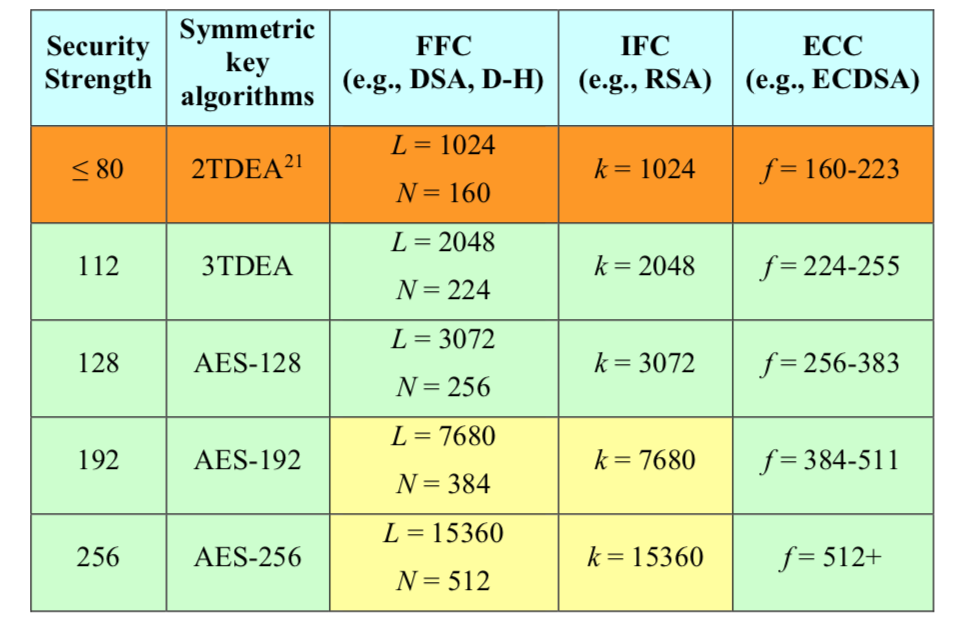
\includegraphics[width=0.9\linewidth]{rsavsecc}
\end{figure*}

\newpage
\section*{Appendix D \hspace{0.5em} ASCII values of most common symbols} \label{app:ascii}
\addcontentsline{toc}{section}{Appendix D \hspace{0.5em} ASCII values of most common symbols}

\begin{figure}[!htb]
	\captionsetup{labelformat=empty}
     \caption{Pattis, Richard E. \textit{ASCII Table}, Carnegie Mellon University, www.cs.cmu.edu/~pattis/15-1XX/common/handouts/ascii.html.}
	 \centering
     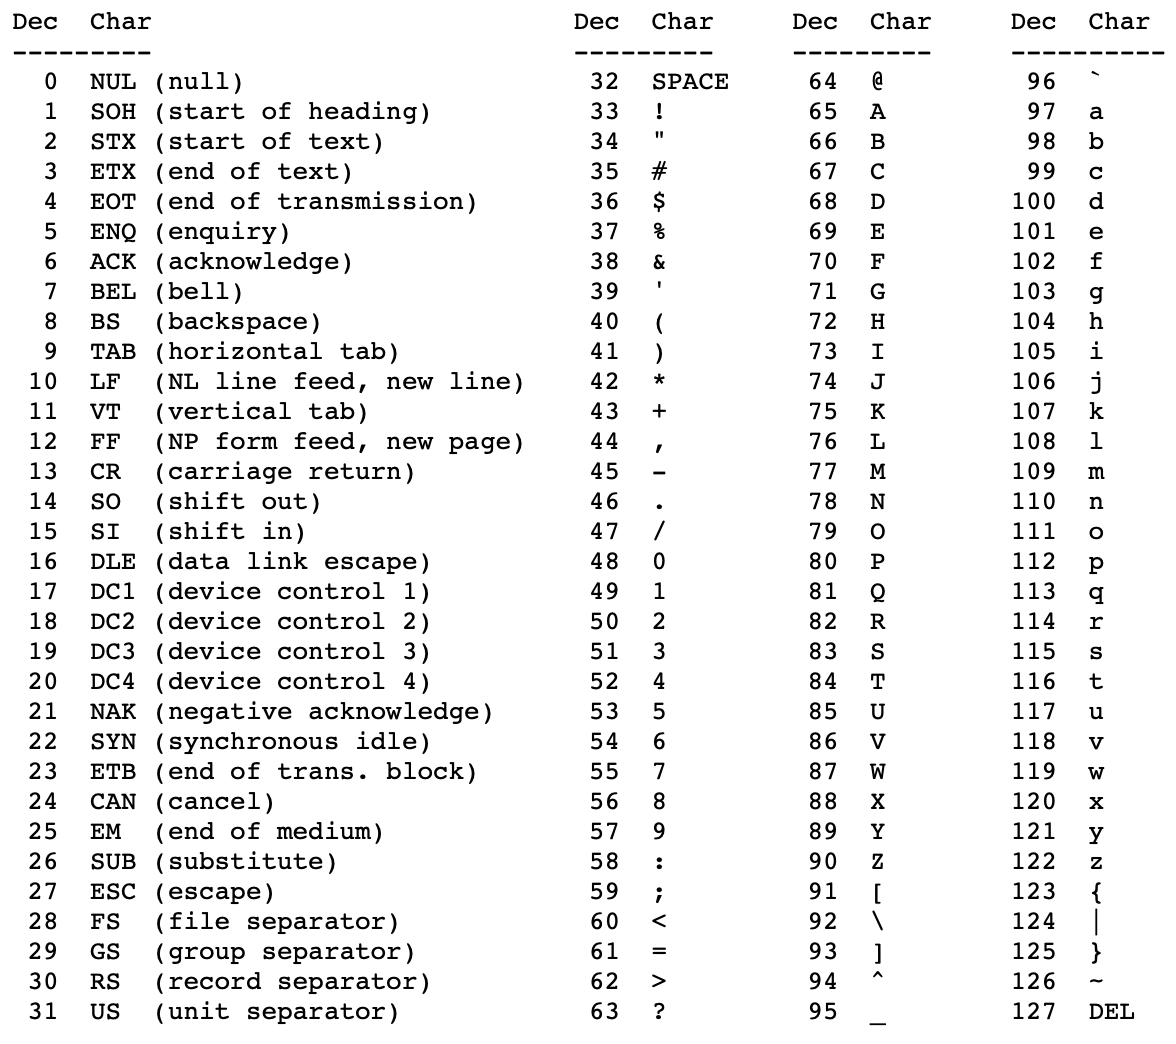
\includegraphics[width=\linewidth]{ascii}
\end{figure}













\end{document}



